\section{Prototype 1}
\label{ap:prototype1}

Afprøvning af Prorotype 1A på Merete er blevet filmet. Klippet kan ses på Youtube: \url{http://youtube.com/watch?v=E-8WA6QrZo4}

Afprøvning af Prorotype 1B på Merete er blevet filmet. Klippet kan ses på Youtube: \url{http://youtube.com/watch?v=rUJexwTpu48}

\begin{description}
\item[Formål] Vores system kan ikke benyttes uden at brugeren indtaster en mængde ingredienser, som de vil udføre en søgning på. For at tilbyde en brugervenlig metode til indtastning af disse ingredienser vil vi gerne teste 2 forskellige metoder på informanterne. Disse 2 metoder testes med hver deres prototype i papirsform, prototype 1A og 1B.
\item[Prototype 1A]

\begin{figure}[H]
\centering
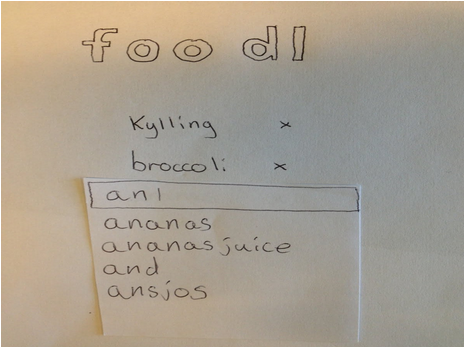
\includegraphics[scale=0.7]{billeder/prototyper/prototype1a.png}
\capt{Visualisering af prototype 1A.}
\label{fig:prototype1a}
\end{figure}

Præsenterer en søgeboks for brugeren, der minder meget om Google’s søgefelt. Når man indtaster et bogstav, fx “k”, kommer der en række forslag frem, såsom kylling og kartoffel, også på samme måde som ved Google, blot med den forskel at der kun foreslås ingredienser. Man kan nu klikke på forslaget eller trykke enter. Man kan også skrive ingrediensens navn færdig manuelt.

Tanken bag denne metode er at man hurtigt kan indtaste en ingrediens hvis man blot ved hvordan de første få bogstaver staves. Brugeren har med stor sandsynlighed kendskab til denne metode, da den bruges af Google, og samtidig har vi også konstrueret logoet og sidens design så det også minder om Google, netop for at gøre det intuitivt for brugeren.

Ulempen er at man har brug for et tastatur og skal tænke over hvordan man staver til ingrediensen. Det er også muligt at overse forslagene og tro man er nødsaget til at stave et meget langt ord, som for eksempel 

\item[Prototype 1B]

\begin{figure}[H]
\centering
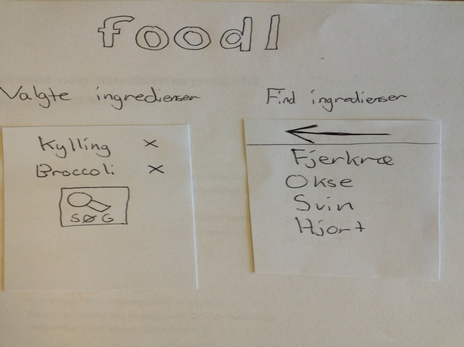
\includegraphics[scale=0.7]{billeder/prototyper/prototype1b.png}
\capt{Visualisering af prototype 1B.}
\label{fig:prototype1b}
\end{figure}

Fokuserer på et valg af ingredienser blandt kategorier. Man vælger først en bred kategori, som for eksempel fjerkræ, kød, brød, frugt og grønt. Dernæst vælger man et antal gange en underkategori, indtil man til sidst kan vælge en ingrediens fra en liste.

Fordelen ved denne metode er at brugeren ikke har behov for et tastatur. Det er også nemt at benytte på tablets og smartphones, da der kan skal klikkes. Ulempen er muligheden for mange kategori og forvirring omkring hvilken kategori en ingrediens findes i. Måske vil den sidste kategori der vælges stadig indeholde rigtig mange ignredienser, sådan at man skal bladre i denne liste for at finde den ønskede ingrediens. 

\item[Sammendrag] Prototype 1A var hurtig, nem og effektiv. Informanten kunne bedst lide denne metode, og hun havde ikke brug for vejledning for at kunne finde de 3 ingredienser kylling, ananas og broccoli.

Prototype 1B var langsommere at bruge og informanten syntes ikke om den. Hun var i tvivl om hvilken kategori hun skulle vælge kylling under. Kategorierne kan laves på mange forskellige måder, og uanset hvordan de vælges, vil der med garanti være nogle brugere der er i tvivl om hvor de skal lede efter en bestemt ingrediens. Et eksempel kan være kartoffelstivelse. Nogle vil lede efter kartoffelstivelse i kategorien grøntsager (fordi kartofler findes der), mens andre måske vil lede efter en kategori med navnet brød og gryn.

På baggrund af informantens valg, vælger vi at benytte metoden fra prototype 1A til at vælge ingredienser.
\end{description}
